\documentclass[twocolumn]{article}

\usepackage{algorithm}
\usepackage{algpseudocode}
\usepackage{graphicx}
\usepackage{amssymb}
\graphicspath{ {./images/} }

%----------TEMP
% \usepackage{xcolor}
% \usepackage{pagecolor}
% \pagecolor{white!5!black!95}
% \color{white!70!black!30}
%----------/TEMP

\title{A GPU based distributed algorithm for HyperNEAT}
\author{Emad Hosseini \thanks{University of Tehran, 
Department of Algorithms and computation.} 
\and Ali Kamandi}

\begin{document}
\maketitle

%----------------------------------------------------

\section{Introduction}

The advancements in the field AI in the past few decades has led to it being one of the tools of our everyday life. Yet there are some great challenges in developing and training AI systems. There are some tasks that today's AI systems are particularly more capable of doing. That includes image classification \cite{DeepImageClassificationReview}, natural language processing \cite{NLPReview}, motor control \cite{DeepRlforMotorControl} and many other fields that previously seemed impossible for machines to do and were considered specific to humans and animals.

But what made these traits possible is the advancements in computers and hardware that made faster processors and larger memories and with the help of more data, scientists could build working AI software. Yet training each model that is capable of a narrow field of tasks takes thousands of hours of CPU time in huge clusters and on sometimes petabytes of data \cite{NEAT-Hardware-IEEE}

Having more data and enough time to process that data is not something to come by easily and in many cases like autonomous navigation in unknown environments or critical decision making for self driving vehicles lack either the data or the time to train conventional neural network models. There are also other challenges including vanishing and exploding gradients \cite{ExplodingAndVanishingGradients}, optimum network structure and other known issues of back propagation that are known to scientists. 

One group of models that tackles these challenges are neuroevolution models. That is defined by Gomez and  Miikkulainen in 1999 as ``systems that evolve neural networks using genetic algorithms'' \cite{NEDefenitionMiikkulainen} and genetic algorithm has some features that makes it ideal for such tasks as training a neural network. These features include no assumptions about the search space and its derivatives, high capability of parallel processing and incremental complexity.

Therefor many research is done in actual models that implement neuroevolution including early works that we mentioned before (\cite{NEDefenitionMiikkulainen}), probabilistic models like the one used by Mao et al. \cite{OtherNESample1}, NEAT \cite{originalNEAT} and many others.

Full utilization of any GA means using its distributable capacities and that is the target of this paper.

In this paper we will introduce a computation method for a specific type of NE model i.e. NEAT using general purpose computers. In the next part we see what has already been done in this field and after that in section 3 our computational method is presented. Some benchmarks are done and results are shown in section 4 with conclusions that follows.

%----------------------------------------------------

\section{Background}

Neuroevolution of augmented topologies (NEAT) is one of the most successful models of neuroevolution introduced in 2002 by Stanley and Miikkulainen \cite{originalNEAT} in this model there is an encoding of the neural network in a genotype that considers an innovation number for each newly formed weight. Also different complexity networks are kept separate using a mechanism of speciation to allow each of them excel in their own rival group and avoid new and unfit individuals get consumed by the older and more mature ones.

A population of such genomes and their respective phenotypes is then created. Using genetic algorithm this population is then directs towards better networks that work better to solve the problem at hand.

NEAT is really successful in finding minimal networks for many tasks that are simple enough but when the requirement of the task is more than that, the search space gets too big and NEAT is inefficient in finding the best networks. This was addressed in another model called HyperNEAT \cite{originalHyperNEAT} that uses underlying symmetries in tasks through a substrate that is essentially a raw initial network.

This substrate is then filled with the connections that are themselves products of another smaller network trained through NEAT algorithm. For example an object detection task would consider the rotation of the target object as a symmetry therefore having a circular substrate leads to automatic consideration of the required symmetry in the task.

The nature of GA involves many simple individuals controlled by an environment that produces the survival of the fittest mechanism for a certain goal. This seems an ideal task for a distributed system. And some researches have already exploited this feature.

for example Such et al. compared using a parallel GPU based and distributed CPU based neuroevolution against other methods of training the network like Q-learning (DQN) and policy gradients (A3C). \cite{GA-GPU-Comparison}

Also the fact that GA can utilize GPU and run more efficient on a distributed systems is not new and many existing research in this field is gathered by Cheng and Gen in their recent review of the field. \cite{GA-GPU-Review}

Using the same methods for getting better results in the HyperNEAT is the target of this paper. There are two main steps in distributing the task of any GA based algorithm the first and easy part is distributing the individuals (which is very important in the case of HyperNEAT as explained in section 3) and the next step is to distribute the control unit that is often called the environment. This part involves each of the separate individuals of the population in the task of finding the fittest and crossover the parents to create child genome replacing them with the less fit individuals.

%----------------------------------------------------

\section{Distributed HyperNEAT}
\label{section:main}
There are a few words that are used in this paper that we should clarify their meaning before we delve into the algorithm. Every neural network problem has vector of real numbers as it's \textit{input} and another vector is generated as \textit{output}. In HyperNEAT there is an empty network that consists only of nodes with no connections which is called \textit{substrate}. The nodes in the substrate have coordinates and it is defined by the expert considering the symmetries and other features of the problem space as defined by Stanley et al. \cite{originalHyperNEAT}

Generally in the literature the genetic algorithm of NEAT is applied on small neural networks with the task of creating best connections for the substrate but in this paper, for the reason which we will discuss later, an \textit{individual} of the genetic algorithm consists of its own copy of the substrate plus, a NEAT genome.

Each individual in this model is capable of generating output based on an input by creating the genotype of NEAT network filling its substrate and running the input vector through the newly generated ANN.

A collection of individuals create a \textit{population} that runs for many \textit{generation}s. Each generation is done by calculating the performance measure for each individual and replacing the unfit ones with the new offsprings of the fitter ones.

\textit{Offspring}s of a generation is the result of \textit{crossover} and \textit{mutation} of existing individuals, the details of which will be addressed later on.

With this terminology we can write the normal HyperNEAT algorithm as in algorithm \ref{alg:HyperNEAT}.

\begin{algorithm}
    \caption{HyperNEAT Algorithm}
    \label{alg:HyperNEAT}
    \begin{algorithmic}[1]
        \Procedure{Train HyperNEAT}{$Inputs$,$Outputs$}
            \State{$Individuals \gets CreateInitialPopulation()$}
            \For {$GenerationCounts$}
                \For{$Individual \in Individuals$}
                    \State{$TotalError \gets 0$}
                    \For{$i \leftarrow 1,|Inputs|$}
                        \State{$Actual \gets GetOutput(Individual,Inputs[i])$}
                        \State{$Error \gets Actual-Outputs[i]$}
                        \State{$TotalError \gets TotalError+Error^2$}
                    \EndFor
                \State{$Error_{Individual} \gets TotalError$}
                \EndFor
                \State{$EvictHighErrors()$}
                \State{$CreateNewChildren()$}
            \EndFor
            \State \Return{$MinErrorIndividual$}
        \EndProcedure
    \end{algorithmic}
\end{algorithm}

We don't go into details of some part of the algorithm here because it's outside the scope of this paper. But one part that interests us is shown in algorithm \ref{alg:Individual}

In algorithm \ref{alg:Individual} $w_{ij}$ is the weight between node $i$ and $j$, $Substrate_{Input}$ is the nodes in the input layer of substrate and likewise, $Substrate_{Output}$ and $Substrate_{Node}$ are respectively output layer nodes and nodes with connection to specified node.

We call this organization of HyperNEAT algorithm as ``CPU version'' from now on but what we actually mean by that is that this runs serially as opposed to ``GPU version'' which will distribute the tasks.

The process in algorithm \ref{alg:HyperNEAT} consists of three parts. The first part is creation of the initial population which is of $\mathcal{O}(n)$ where $n$ is size of the population. Because creating each individual takes constant time for each of the NEAT genomes as each one contains exactly $2d$ randomized weights where $d$ is the number of dimensions specifying coordinated of a node in the substrate. For example a 2D grid substrate will have a 2D coordinate position for each node and the substrate would have 4 input nodes taking in 2 nodes and giving back the weight between them.

The third part of the algorithm \ref{alg:HyperNEAT} is the eviction and recreation of next generation. The eviction percentage of the total population is another parameter of the algorithm. Creating a next generation individual from existing ones is not deterministic and involves two stochastic steps of cross-over and mutation. We will not go through this analysis in this paper and generally the third part is $\mathcal{O}(geE_c)$ where $g$ is the number of generations, $e$ is number of evictions and $E_c$ is the expected value of time requirement of the creation of a new individual with cross-over and mutation operations.

The second part of algorithm \ref{alg:HyperNEAT} is the actual training generations which we will focus on. The time complexity of this part of the  algorithm \ref{alg:HyperNEAT} is heavily dependant on the time complexity of algorithm \ref{alg:Individual} which is not deterministic due to the stochastic nature of the NEAT algorithm.

\begin{algorithm}
    \caption{Calculate output for each individual}
    \label{alg:Individual}
    \begin{algorithmic}[1]
        \Procedure{GetOutput}{$Individual$,$Input$}
            \State{$NEAT = CreatePhenotype(Genome_{Individual})$}
            \For{$Node_i \in Substrate$}
                \For{$Node_j \not= Node_i \in Substrate$}
                    \State{$w_{ij}=GetOutput_{NEAT}(Node_i,Node_j)$}
                    \If{$w_{ij}<Threshold$}
                        \State{$w_{ij}=0$}
                    \EndIf
                \EndFor
            \EndFor
            \For{$Node \in Substrate_{Input}$}
                \State{$Value_{Node} \gets Input_i$}
            \EndFor
            \For{$Node \in Substrate_{Output}$}
                \State{$GetValueRecursive(w,Node)$}
            \EndFor
            \State \Return{$Substrate_{Output}$}
        \EndProcedure
        \Procedure{GetValueRecursive}{$w$,$Node$}
            \If{$Value_{Node} \not= null$}
                \State \Return{$Value_{Node}$}
            \EndIf
            \State{$sum \gets 0$}
            \For{$ConnectedNode \in Substrate_{Node}$}
                \State{$value \gets GetValueRecursive(ConnectedNode)$}
                \State{$sum \gets sum + value \times w_{ij}$}
            \EndFor
            \State{$Value_{Node} \gets ApplyActivation(sum)$}
            \State \Return {$Value_{Node}$}
        \EndProcedure
    \end{algorithmic}
\end{algorithm}

Let $E_I$ be the unknown expected time complexity of getting the output of a single individual for a single input. Then $\mathcal{O}(gnTE_I)$ will be the time complexity of the second part of algorithm \ref{alg:HyperNEAT} where $T$ denotes the number of training data size.

The total time complexity of the algorithm \ref{alg:HyperNEAT} is shown in equation \ref{eq:CPUTime}.

\begin{equation}
    \label{eq:CPUTime}
    \mathcal{O}(n+gnTE_I+geE_c)
\end{equation}

\subsection{Thread per Individual}

As it is clear in algorithm \ref{alg:HyperNEAT} in previous section, training phase of the HyperNEAT consists of a 3 layer main loop. These loops can be addressed by parallelism to reduce time complexity of the algorithm.

We will first combine the inner two loops in a collection of single operations. Each of these operations will calculate the actual error of a single input for a single individual. This simple process is shown in algorithm \ref{alg:parallel1}.

\begin{algorithm}
    \caption{Kernel of the parallel mode}
    \label{alg:parallel1}
    \begin{algorithmic}
        \State{$Actual \gets GetOutput(Individual,Inputs[i])$}
        \State{$Error \gets Actual-Outputs[i]$}
        \State{$TotalError \gets TotalError+Error^2$}
    \end{algorithmic}
\end{algorithm}

There are many memory operations done in single machine (i.e. CPU) mode of the algorithm that we ignored for simplicity but, for the sake of completeness we will include the amount of added memory operations to the multi-machine (i.e. GPU) mode. Since the internal operations between the two modes are the same read and write access to memory is the same in both modes. The only added memory operations are the necessary data transfer required for data integrity and reading the results, between the machines in the multi-machine mode.

Another thing worth mentioning here is that there will be a controller (leader) machine in multi-machine mode. In our particular architecture of using a CPU and many processors of the GPU as the cluster machines the CPU will play the role of the leader.

Getting back to algorithm \ref{alg:parallel1}, execution requires $n.T$ single operations in general there will be $m$ machines where $m<n$ and since $T>1 \Rightarrow m<n.T$. So we split the required error value calculation of each generation into chunks of size shown in equation \ref{eq:SizeOfmMachines}.

\begin{equation}
    \label{eq:SizeOfmMachines}
    \Bigl\lfloor \frac{n.T}{m} \Bigr\rfloor    
\end{equation}

This way the $nT$ in the middle part of equation \ref{eq:CPUTime} will be replaced by the value in equation \ref{eq:SizeOfmMachines}. But the data must be transferred to cluster machines. The required data for algorithm \ref{alg:parallel1} is the individual and the input. The input is fixed in size and it's size is negligible asymptotically compared to the individual. The individual size is in direct order of the time required for it to get a single output and therefore $\mathcal{O}(Individual)=E_I$ which is unknown but by placing these values in equation \ref{eq:CPUTime} we will get the time complexity of the algorithm as in equation \ref{eq:GPUTime}.

\begin{equation}
    \label{eq:GPUTime}
    \mathcal{O}(n+g \frac{nT}{m}E_I+nE_I+geE_c)=\\
    \mathcal{O}(n+nE_I(\frac{gT}{m}+1)+geE_c)
\end{equation}

This is the time reduction for fixed amount of stochastic training that NEAT offers and simply means more training in the same time. But one more implication of this statement is that with this method you can have more individuals in the population which by the mechanism of speciation causes more young species. The speciation mechanism is the counterpart of exploration as oppose to inter-species exploitation of GA algorithm and a good ballance in the two can be achieved in this algorithm where you can have more individuals. \cite{ExploreVsExploit}

In equation \ref{eq:GPUTime} if we increase the number of population, $n$, and the number of machines, $m$, since $E_I$ will remain constant, we will see a factor of $1/m$ decrease in time complexity of the algorithm.

\subsection{Distribution Challenges}
The original NEAT and HyperNEAT algorithms were not designed with distributed environment in mind. Although, as mentioned in previous section, genetic algorithms have a natural tendency to be used in distributed architecture, some challenges arose in the implementation of this particular algorithm for GPU.

First one is the innovation number. Innovation number is a mechanism originally included in NEAT algorithm to be incorporated with each network connection and provide the ability to distinguish similar and different connections even when the nodes and weights of them have mutated over time. \cite{originalNEAT}

Assigning a number for this innovation number is an easy task in single process architecture but, not in distributed architecture. We should notice that the intentions behind innovation number only requires a unique id and the order of that is not important for the algorithm. Therefore we have assigned innovation numbers not based on a simple increasing number but as a combination of process id and a number generated in each process.

One more thing that plagued our particular implementation is the matter of using device bandwidth in moving data from CPU to GPU. This might not effect the more broad multi-machine usage of this algorithm but, in single machine CPU-GPU implementation that we use moving data to and from GPU has a overhead cost of opening and closing the stream.

To handle this issue we split the operation in two parts first we move all required data to GPU memory and then access it in different threads. This does not have an effect on our complexity analysis but extremely improves performance in wall clock time of algorithm execution due to removal of I/O waits and utilizing device bandwidth.

% Recursion limitation in GPU

%----------------------------------------------------

\section{Comparison of Results}
In this study we have used nVidia CUDA\textsuperscript \textregistered library which is well known and widespread in the GP-GPU community. The program is written in C++ in a way that the same code runs on the CPU as in algorithm \ref{alg:HyperNEAT} as well as GPU. The benchmarks will therefore not include implementation differences of the two platforms.

Selected task is also a very simple function approximation task, since the performance of both algorithms will be the same in terms of accuracy and the goal is speed improvement.

The data-set consists of 10,000 randomly generated 2D inputs in the form of $[x,y]$ where $x,y \in \mathbb{R}$ and $0<x,y<100$. 80\% of this data is used for training and the rest used for test phase. The expected output is $z$ as shown in equation \ref{eq:ExpectedOutput}. In which $\epsilon$ is white noise introduced to make the problem more challenging.

\begin{equation}
    \label{eq:ExpectedOutput}
    z=x^2+y^2+\epsilon \quad \epsilon \sim N(0,1)
\end{equation}

The value of $m$ is defined by the system and there is little control over it. The test results shown here are generated using a \textit{nVidia GeForce GTX 960m} with 640 CUDA cores and 4GB of memory. Also host computer (which runs the CPU tests) has an \textit{Intell Core i7 6700HQ} processor.

Number of individuals, $n$, and generations, $g$ however are configuration parameters and can be changed easily. $T$ and $e$ are dictated by the data-set and we will not change them in our analysis for better comparisons.

\begin{figure*}
    \centering 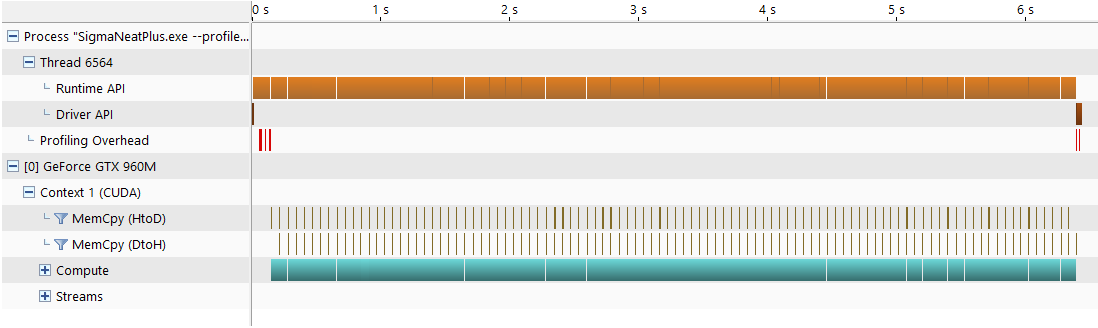
\includegraphics[width=\textwidth]{ProfiledSingleGenerationOf100}
    \caption{Profiler output of parallel algorithm}
    \label{img:profiler}
\end{figure*}

The chart shown in figure \ref{img:profiler} shows how much parallel work has been done. This is the result of 1 generation of $n=100$ individuals ran in around 6.4 seconds\footnote{The overhead of the profiler tool is included in these measurements.}. The same configuration runs around 7.7 seconds in CPU.

If we keep increasing the value of $n$ and track the runtime of the application for one generation, we expect the time to increase with each new individual added to the population but there will be two constant factors. One is the amount CPU works needed for each generation i.e. for eviction, initial creation of individuals, reading training data from file and etc. and the second is the time required to transfer data to and from GPU.

\begin{figure*}
    \centering 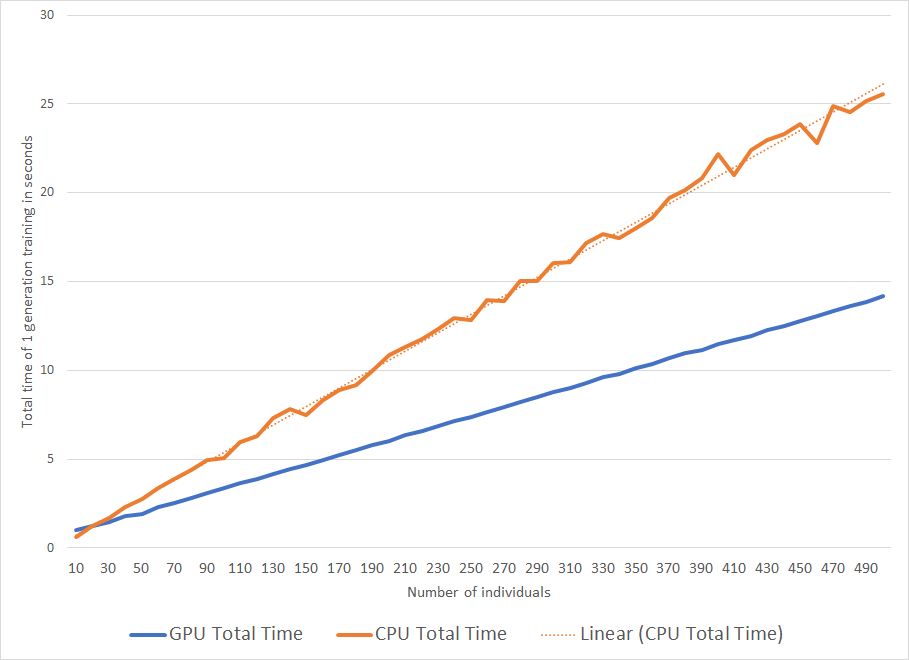
\includegraphics[width=\textwidth]{IndivTotal}
    \caption{Comparison of total training time of 1 generation of $n$ individuals}
    \label{img:IndivTotal}
\end{figure*}

The chart in figure \ref{img:IndivTotal} shows the result that we expected. In it, the amount of time required for a single training generation of different sizes of population is shown for both CPU and GPU versions of the algorithm.

At first the GPU transfer time is causing the total time of GPU to be higher than CPU but as the population size increases, this time dissipates and parallel execution of individuals runs around 2 times faster at $n=500$. The CPU work overhead is constant for both scenarios. Later we will give an idea about how we can distribute that work between different processors as well.

\begin{figure*}
    \centering 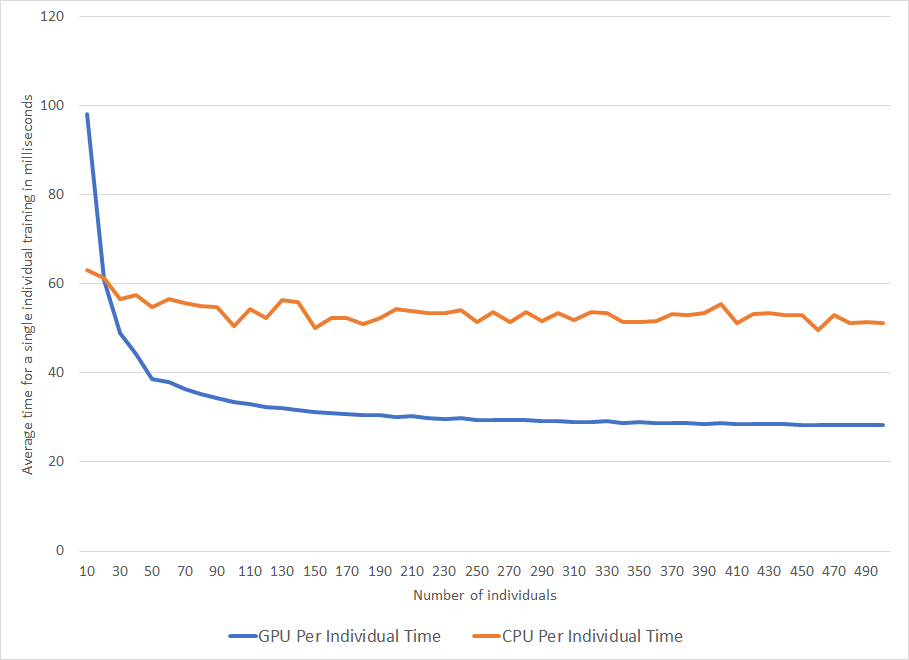
\includegraphics[width=\textwidth]{IndivSingle}
    \caption{Comparison of average training time of 1 individual for 1 generation}
    \label{img:IndivSingle}
\end{figure*}

The effect of the transfer overhead can be seen in figure \ref{img:IndivSingle}. In that the average time of running a single individual is shown for both GPU and CPU models. At first in lower population sizes GPU takes around double the time of CPU for calculating the output of each individual then, a sharp drop happens and the situation changes. This drop virtually does not exist in CPU version.

One observation that you might have is the difference between the smoothness of the charts. The smoothness of results for GPU in both figures is duo to the fact that GPU is a collection of processors and that averages the result of each. The performance of each processor may have fluctuations like we see in CPU charts. These results are the average of 3 runs per each scenario.

The results in figure \ref{img:IndivTotal} doesn't show the actual difference between the two approaches. Because it ran for only 1 generation and an important part of the algorithms, i.e. the eviction of old and creating new individuals, is left out. If we run the algorithm for longer we will see that, since most of the execution time is used for the second part of algorithm \ref{alg:HyperNEAT} the same result will hold.

For example running the algorithm for 100 generations of 100 individuals for 3 times is done in average 285.530s in GPU and 511.398s in CPU which shows about 56\% increase in performance. And the gap will only widen as $n$ and $g$ increase.

%----------------------------------------------------

\section{Conclusion}

In this paper we have introduced a parallel mechanism to run an existing neuroevolution algorithm. We have overcome the challenges and ran the algorithm on GPU using nVidia CUDA technology. But as we kept this mindset throughout the paper this algorithm can run on any distributed processor system and gain an even greater performance gain.

The actual goal here was to give a mechanism for scaling the neuroevolution approach for training neural networks. Since most of the research in ANNs is done using back propagation algorithm which scales well but, limits the search space only to smooth and derivable activation functions.

The proposed algorithm showed scalability of the algorithm to almost double the performance of the conventional implementations.

%----------------------------------------------------

\section{Future Studies}

The distributed algorithm described in section \ref{section:main} has the benefit of breaking the main loop. While in theory we should be able to distribute each individual for itself.

This requires a communication model between the individuals that doesn't have a huge impact on the total working time of each of them. Also as mentioned before there are many tasks involved in the population control that needs to be addressed by a central node. This node can certainly use the leader election algorithms like \cite{LeaderElection1} and \cite{LeaderElection2}.

This higher level of distribution can be considered as future goals of such development.

%----------------------------------------------------

\bibliographystyle{unsrt}
\bibliography{bibiliography}

\end{document}
